\newpage
\section{Further results and discussion}
The transverse momentum distributions of double-strange hyperon resonances, \xis, produced in p--Pb collisions at \snn = 5.02 TeV and Pb--Pb collisions at \snn = 2.76 TeV were measured in the mid-rapidity range and they have been already presented in Chapter \ref{sec:pPbPbPb}. From the measurement, the $\mpt$ and integrated particle yield ratios with system size have been obtained. In the present Chapter these results are compared with model predictions and discussed in connection with the following topics: 

\begin{itemize}
\item Mean transverse momentum studies
\item Study of particle production mechanism in hadronic phase
\item Study of strangeness enhancement
\end{itemize}

Most of the theoretical aspects related to these topics and, in particular, the description of the models already have been adrressed in Chapter \ref{sec:model}.


% The mean transverse momentum values are presented as a function of $\meandNdeta$, as well as a function of the particle masses and compared with previous results on hyperon production. The integrated yield ratios of excited to ground-state hyperons are constant as a function of $\meandNdeta$. The equivalent ratios to pions exhibit an increase with $\meandNdeta$, depending on their strangeness content.


\subsection{Mean transverse momentum}

Figure~\ref{fig:mean_pt_vs_mult} shows the mean transverse momentum $\mpt$ as a function of mean 
charged-particle multiplicity density $\langle$d$N_{\mathrm{ch}}$/d$\eta_{\mathrm{lab}}\rangle$ at midrapidity.
The results for \xis are compared with those for other hyperons observed in p--Pb collisions at \snn = 5.02~TeV~\cite{cite:lambda_pPb, cite:Xi_pPb}.

\begin{figure}[htbp]
\begin{center}
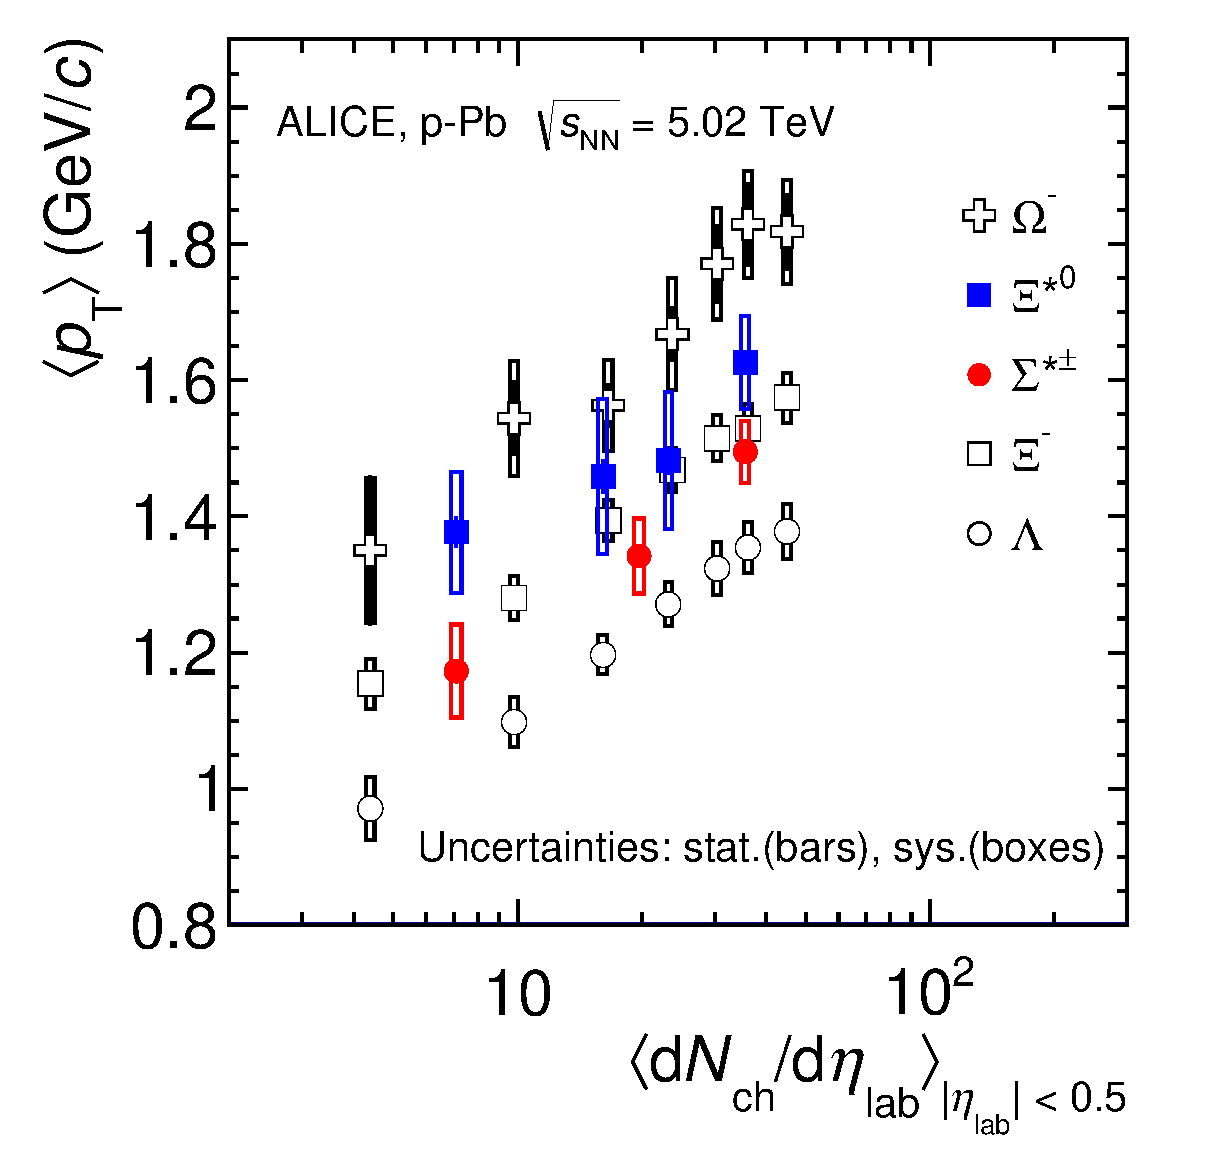
\includegraphics[width=10.cm]{./Version1/FigChapter6/mpt/mpt_mult.eps}
\caption{Mean transverse momenta $\mpt$ of $\Lambda$, $\Xi^{-}$, $\Sigma^{*\pm}$, $\Xi^{*0}$ 
  and $\Omega^{-}$ in p--Pb collisions at \snn = 5.02 TeV as a 
  function of mean charged-particle multiplicity density 
  $\langle$d$N_{\mathrm{ch}}$/d$\eta_{\mathrm{lab}}\rangle$, measured in the pseudorapidity range 
  $\mid\eta_{\mathrm{lab}}\mid <$~0.5. The results for $\Lambda$, $\Xi^{-}$ and $\Omega^{-}$ are taken 
  from~\cite{cite:lambda_pPb, cite:KphipPb, cite:Xi_pPb}. Statistical and systematic uncertainties are represented as bars 
  and boxes, respectively. The $\Omega^-$ and $\Xi^-$ points in the 3rd and 4th lowest multiplicity bins are slightly 
  displaced along the abscissa to avoid superposition with the \xis points.}
  \label{fig:mean_pt_vs_mult}
  \end{center}
\end{figure}


Increasing trends from low to high multiplicities are observed for all hyperons. The mean transverse momenta increase by 20\% as the mean charged-particle multiplicity increases from 7.1 to 35.6. This result is similar to the one obtained for the other hyperons. Furthermore, a similar increase has been observed also for K$^{\pm}$, K$_{\rm{S}}^{0}$, K$^{*}(892)^0$ and $\phi$~\cite{cite:KphipPb}, whereas protons are subject to a larger ($\sim$ 33\%) increase in the given multiplicity range, as discussed also in Ref.~\cite{cite:lambda_pPb}. 


\begin{figure}[htbp]
\begin{center}
\includegraphics[width=10.cm]{./Version1/FigChapter6/mpt/mpt_mass.eps}
\caption{Mass dependence of the mean transverse momenta of identified particles for the $0-20$\% V0A multiplicity class and with $-0.5<y_{\mathrm{CMS}}<0$ in p--Pb~collisions at \snn = 5.02 TeV~\cite{cite:lambda_pPb, cite:Xi_pPb}, and 
  in minimum-bias pp collisions at $\sqrt{s}$~=~7~TeV~\cite{cite:Xi_pp} with $|y_{\mathrm{CMS}}|<0.5$. Additionally, $D^0$ and $J$/$\psi$ results are plotted. The $D^0$ and $J$/$\psi$ were measured in different rapidity ranges: $|y_{\mathrm{CMS}}|<0.5$~\cite{cite:D0} 
  ($|y_{\mathrm{CMS}}|<0.9$~\cite{cite:Jpsi_pp}) for $D^0$ ($J$/$\psi$) in pp and $-0.96 < y_{\mathrm{CMS}}< 0.04$~\cite{cite:D0} ($-1.37<y_{\mathrm{CMS}}<0.43$~\cite{cite:Jpsi_pPb}) 
  for $D^0$ ($J$/$\psi$) in p--Pb. Note also that the results for $D^0$ and $J$/$\psi$ in p-Pb collisions are for the 0-100\% multiplicity class.}
  \label{fig:mean_pt_vs_mass}
 \end{center}
\end{figure}

In all multiplicity classes, the $\mpt$ follows an approximate mass ordering:  
\begin{itemize}
\item $\mpt_{\Lambda}<\mpt_{\Xi^-}$~$\simeq$~$\mpt_{\Sigma^{*\pm}}<\mpt_{\Xi^{*0}}<\mpt_{\Omega^{-}}$ 
\end{itemize}

The $\mpt$ of $\Sigma^{*\pm}$ looks systematically lower than the $\mpt$ of $\Xi^{-}$, despite the larger mass of 
$\Sigma^{*\pm}$. The uncertainties, however, are too large to draw any conclusion on 
possible hints of violation of the mass hierarchy. This hierarchy of mass-ordering, also including $D^0$ and 
$J$/$\psi$ in the comparison, is displayed in Figure \ref{fig:mean_pt_vs_mass}. Note, however, that the $D^0$ and $J$/$\psi$ were 
measured in different rapidity ranges: $|y_{\mathrm{CMS}}|<0.5$~\cite{cite:D0} ($|y_{\mathrm{CMS}}|<0.9$~\cite{cite:Jpsi_pp}) for $D^0$ ($J$/$\psi$) in pp and $-0.96 < y_{\mathrm{CMS}}< 0.04$~\cite{cite:D0} ($-1.37<y_{\mathrm{CMS}}<0.43$~\cite{cite:Jpsi_pPb}) for $D^0$ ($J$/$\psi$) in p--Pb, and the results for $D^0$ and $J$/$\psi$ in p-Pb collisions are for the 0-100\% multiplicity class. This mass dependence is observed in both p--Pb and pp collisions. 
It was observed also by the STAR collaboration~\cite{cite:STAR-hadronic_resonances-dAu} in MB pp, MB d--Au and central Au--Au collisions. 

Furthermore, for the light-flavour hadrons, the mean transverse momenta in p--Pb collisions are observed to be consistently higher than those in pp collisions at 7 TeV. The situation for the charm hadrons is different, where $\mpt$ appears compatible between both colliding systems. The discrepancy is likely due to different production mechanisms for heavy and light flavours and to a harder fragmentation of charm quarks. Specifically, the fact that $\mpt$ remains similar in pp and in p--Pb is consistent with an $R_{\mathrm{pPb}}$ ratio compatible with unity at all \pt \cite{cite:D0} for $D^0$, and/or 
with the effects of shadowing in p--Pb which reduces the production at low \pt and thus increasing the overall $\mpt$ for $J$/$\psi$~\cite{cite:Jpsi_pPb}; the small \pt hardening expected in pp when going from 5.02 to 7TeV is apparently not enough to counter-balance the situation.

Because of small decrease of the $\mpt$ for proton and $\Lambda$ relative to those for K$^{*0}$ and $\phi$, two different trends for mesons and baryons have been suggested~\cite{cite:mass_scaling}. Even including $D^0$ and $J$/$\psi$, as shown in Figure ~\ref{fig:mean_pt_vs_mass}, a different trend for 
mesons and baryons cannot be convincingly established.


%%%%
\newpage
\subsection{Particle yield ratios}
\subsubsection{Integrated yield ratios of excited to ground-state hadrons}

The integrated yield ratios of excited to ground-state hyperons \cite{cite:pp7_multistrange, cite:lambda_pPb, cite:Xi_pp, cite:Xi_pPb} 
with the same strangeness content, for different collision systems and energies, are shown in Figure \ref{fig:xitoxi} as a function of system size. The ratio of \xis to $\Xi$ is flat across the system and it complements the information derived from other resonance measurement for different lifetime which are shown in Figure \ref{fig:rsnratio}.


The short-lived resonances($\rho$, K* and $\Lambda$*) which exhibit suppression from peripheral to central lead-lead collisions and with respect to thermal model in central lead-lead collisions. Currently favored explanation of  is dominance of elastic re-scattering of decay daughters over regeneration in the hadronic phase.

The constant behavior of the yield ratios of excited to ground-state hyperons with same strangeness content (\xis and $\Phi$) indicates that neither regeneration nor re-scattering dominates with increasing collision system size because of its longer-lifetime.

\begin{figure}[htbp]
\begin{center}
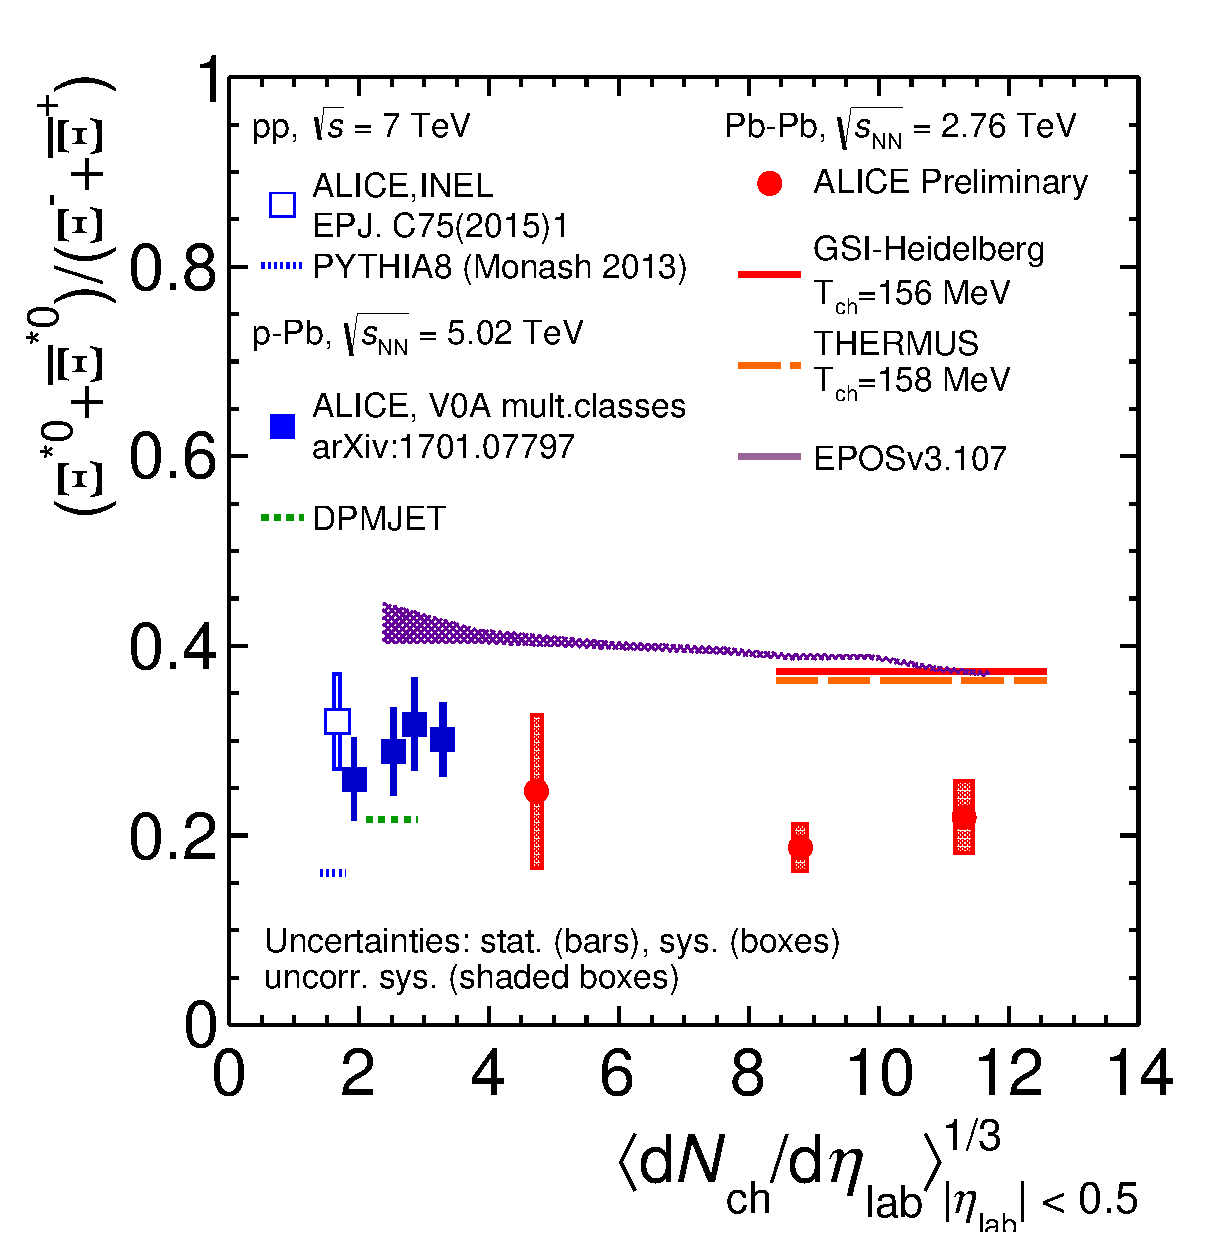
\includegraphics[width=10.cm]{./Version1/FigChapter6/Ratio/Ratio_XiStarToXi}
\caption{Ratio of \xis to $\Xi^-$ measured in pp \cite{cite:Xi_pp}, p--Pb \cite{cite:lambda_pPb, cite:Xi_pPb}  and Pb--Pb collisions as a function of $\langle$d$N_{\mathrm{ch}}$/d$\eta_{\mathrm{lab}}\rangle$ measured at midrapidity. Statistical uncertainties (bars) are shown as well as total systematic uncertainties (hollow boxes) and systematic uncertainties uncorrelated across multiplicity (shaded boxes). A few model predictions are also shown as lines at their appropriate abscissa.}
\label{fig:xitoxi}
\end{center}
\end{figure}

\begin{figure}[htbp]
\begin{center}
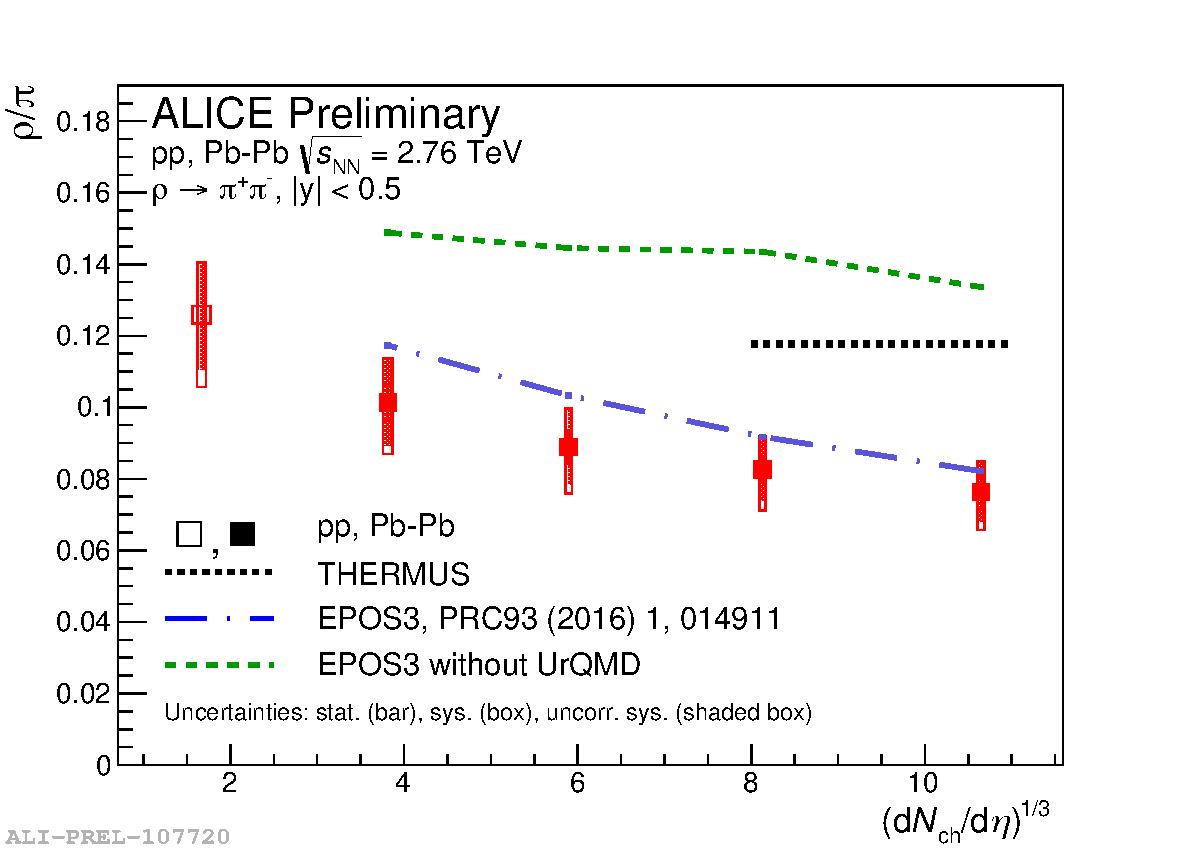
\includegraphics[width=8.cm]{./Version1/FigChapter6/Ratio/RhoRatio}
\hspace{0.5cm}
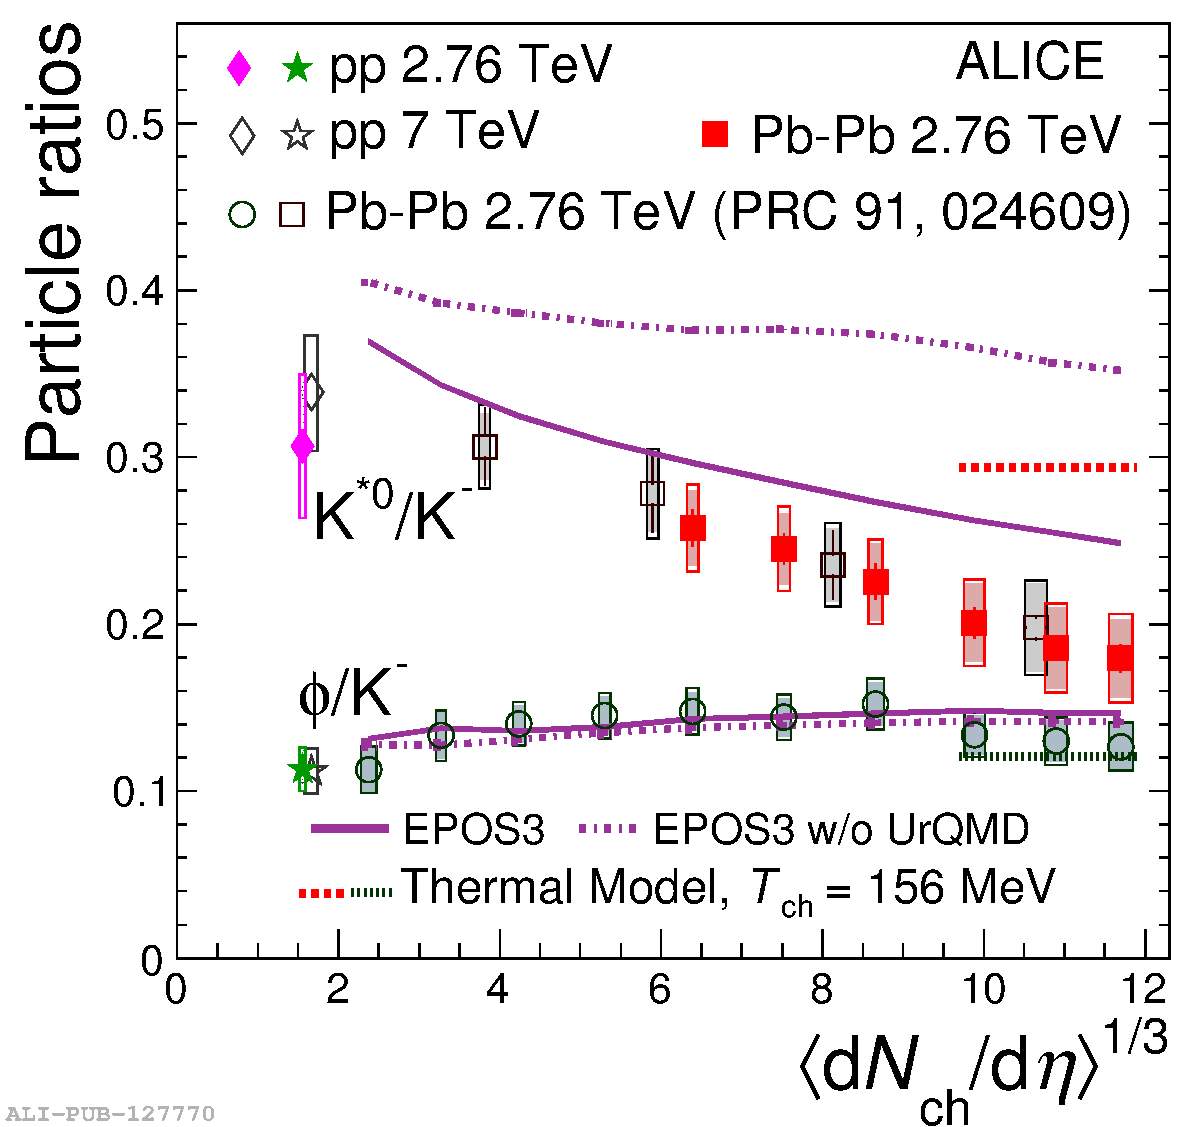
\includegraphics[width=7.cm]{./Version1/FigChapter6/Ratio/KPhiRatio}
\hspace{0.5cm}
\includegraphics[width=7.cm]{./Version1/FigChapter6/Ratio/LambdaRatio}
\caption{Ratio of $\rho$/$\pi$(Up), K*/K, $\phi$/K(Left bottom) and $\Lambda*$/$\Lambda$ with system size measured at mid-rapidity. Statistical uncertainties (bars) are shown as well as total systematic uncertainties (hollow boxes) and systematic uncertainties uncorrelated across multiplicity (shaded boxes). A few model predictions are also shown as lines at their appropriate abscissa.}
\label{fig:rsnratio}
\end{center}
\end{figure}

%%

\newpage
\subsection{Integrated yield ratios to pion}
The integrated yield ratios of excited hyperons to pions are shown in Figure \ref{fig:xitopi} to study the evolution of relative strangeness production yields with increasing collision system size. The ratio of \xis to $\Xi$ is observed to be increase from pp to p--Pb collisions system and then, decrease from peripheral to central Pb--Pb collision. The QCD-inspired predictions like PYTHIA for pp \cite{cite:pythia8} and DPMJET for p--Pb~\cite{cite:DPMJET} clearly underestimate the observed yield ratios, while the statistical one seems to be comparable with results from high multiplicity in p--Pb but the ratio in Pb--Pb is below with respect to the model. 
The results in pp and p--Pb collisions are consistent with previous observation of ground-state hyperons to pion ratios. The Figure \ref{fig:doubler} presents particle yield ratios to pions of strange and multi-strange hadrons normalized to the values measured in pp collisions. As shown in the Figure \ref{fig:doubler}, the \xis to pion ratios follow the trend of $\Xi$\ $\pi$ as function  of $\meandNdeta$ and indicate that the strangeness enhancement observed in p--Pb collisions depends predominantly on the strangeness content, rather than on the hyperon mass. 

%The Figure \ref{fig:topi} also shows the hyperon-to-pion ratios and compared with model predictions. 


\begin{figure}[htbp]
\begin{center}
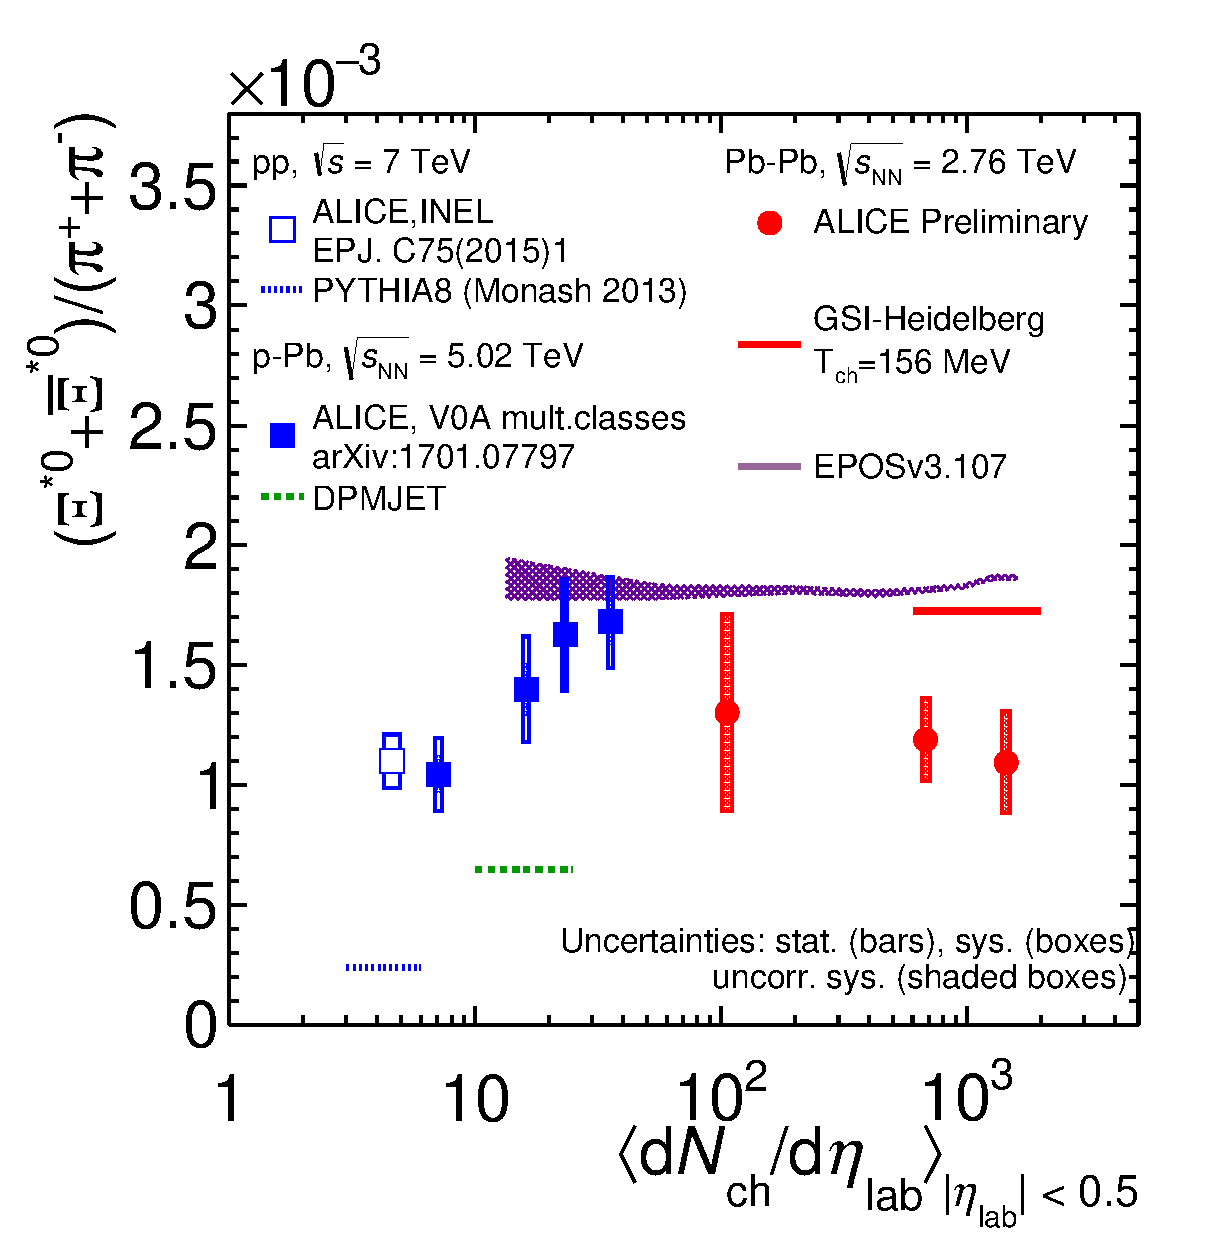
\includegraphics[width=10.cm]{./Version1/FigChapter6/Ratio/Ratio_XiStarToPion}
\caption{Ratio of \xis to $\pi^{\pm}$, measured in pp \cite{cite:pp7_piKp} and p--Pb \cite{cite:Xi_pp} collisions, as a function of the average charged particle 
 density ($\langle$d$N_{\mathrm{ch}}$/d$\eta_{\mathrm{lab}}\rangle$) measured at mid-rapidity. Statistical uncertainties (bars) are shown as well as total systematic uncertainties (hollow boxes) and systematic uncertainties uncorrelated across multiplicity (shaded boxes). A few model predictions are also shown as lines at their appropriate abscissa.}
\label{fig:xitopi}
\end{center}
\end{figure}

\begin{figure}[htbp]
\begin{center}
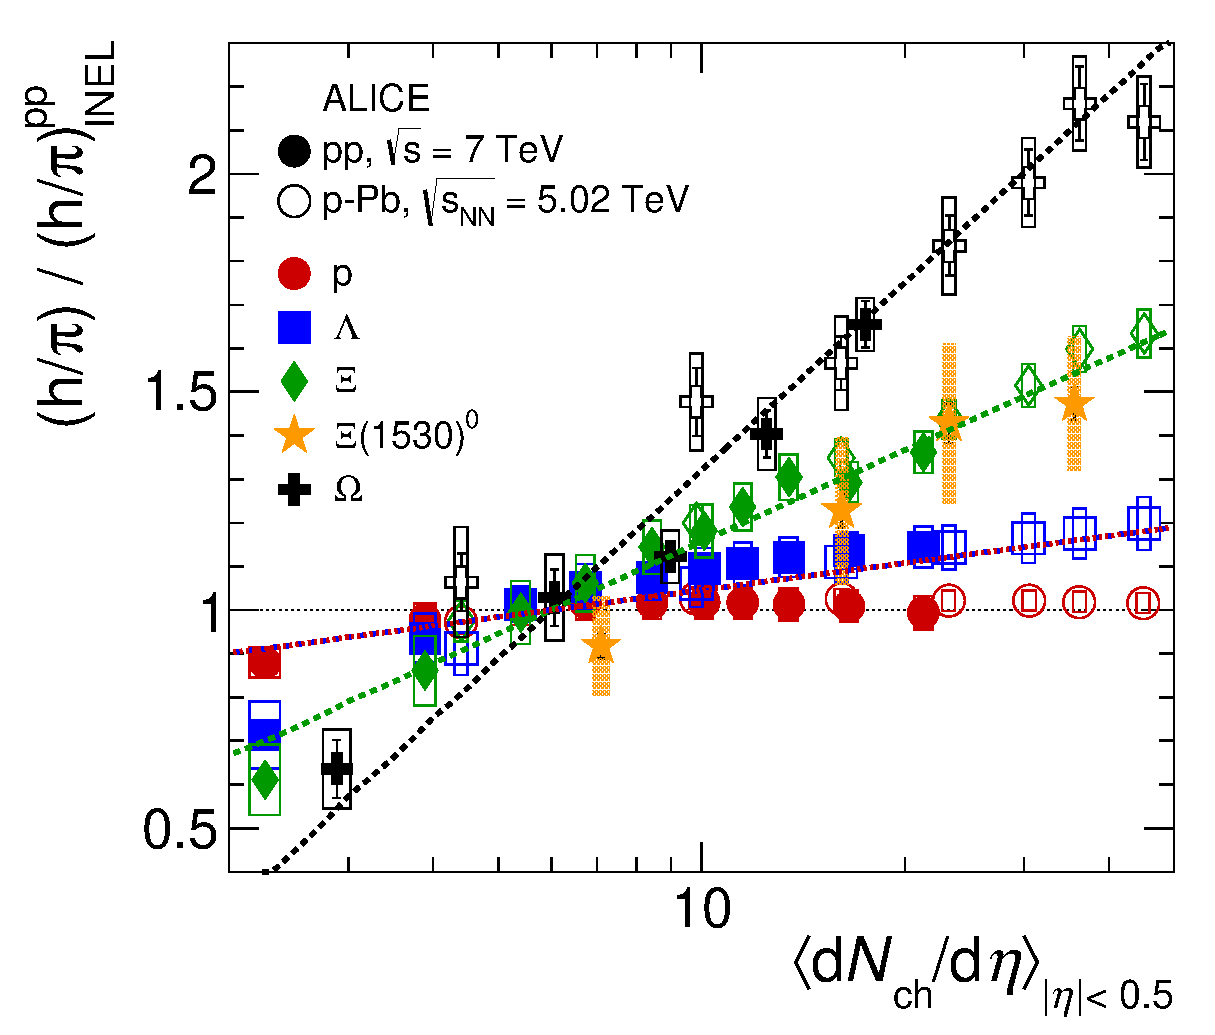
\includegraphics[width=10.cm]{./Version1/FigChapter6/Ratio/RatioToPionXiStar}
\caption{ Particle yield ratios to pions of strange and multi-strange hadrons normalized to the values measured in pp collisions, both in pp and in p--Pb collisions. The common systematic uncertainties cancel in the double-ratio. The empty boxes represent the remaining uncorrelated uncertainties. %The lines represent a simultaneous fit of the results with the empirical scaling formula in Equation~\ref{eq:scaling}.
}
\label{fig:doubler}
\end{center}
\end{figure}


%\begin{figure}[htbp]
%\begin{center}
%\includegraphics[width=10.cm]{./Version1/FigChapter6/Ratio/RatioToPion}
%\caption{ \pt-integrated yield ratios of strange and multi-strange hadrons to ($\pi^{+}+\pi^{-}$) as a function of $\meandNdeta$ measured in the rapidity interval $|\eta|<$ 0.5. The empty and dark-shaded boxes show the total systematic uncertainty and the contribution uncorrelated across multiplicity bins, respectively. The values are compared to calculations from MC models and to results obtained in Pb--Pb and p--Pb collisions at the LHC.}
%\label{fig:topi}
%\end{center}
%\end{figure}



\newpage
%\subsubsection{Comparison with other resonances}
%\subsubsection{Comparison with models}